\documentclass[solution, letterpaper]{cs121}

\usepackage{tikz-qtree}
\usepackage{graphicx}

%% Please fill in your name and collaboration statement here.
%\newcommand{\studentName}{Renzo Lucioni and Daniel Broudy}
%\newcommand{\collaborationStatement}{I collaborated with...}
\newcommand{\solncolor}{red}
\begin{document}

\header{X}{May 9, 2013, at 23:59}{}{}

%%%%%%%%%%%%%%%%%%%%%%%%%%%%%%%%%%%%%%%%%%%%%%%%%%%%

\section*{Overview}
\hspace{4mm} We chose to use an artificial neural network, a finite memory policy, and Q-learning to implement our player for the final project. The following writeup describes the motivation behind using each of these methods, explains our design of each method, and discusses the application of each method in the context of playing the game. We then evaluate the performance of each method.

\section{Artificial Neural Network}
\subsection{Motivation}
\hspace{4mm} When our player requests a plant observation, it receives a noisy image. The player must be able to determine, with a reasonable degree of confidence, whether a nutritious or poisonous plant is depicted in the image. As we learned in Homework 2, a multi-layer feed-forward neural network is a good approach to image classification, superior to decision trees, boosted decision stumps, and perceptrons. Like perceptrons, multi-layer feed-forward neural networks are capable of making use of all pixels in an image, allowing them to learn the relationships between pixels. However, unlike perceptrons, neural networks can also use hidden layers to recognize non-linearly separable functions. This allows neural networks to recognize rotations, translations, and skews (i.e., noise) that would have defeated a perceptron. Thus, neural networks are both accurate and robust when determining the class of an input image, whether it be a digit or a plant. As such, we chose to train a neural network in order to give our player the ability to better distinguish between plant images.

\subsection{Design}
\hspace{4mm} In order to train a neural network, we first need access to classified training instances. We collected this training data by sampling the images generated throughout the course of normal gameplay by the stock random players. These default players always consume a plant if one is present at their current location after requesting 5 observations of it. We extracted images from the game by writing the image tuples returned by the {\tt GetImage()} method to a file. We determined labels for these stored image tuples by calculating the difference in life points before and after eating the plant they came from. For convenience, we set the plant bonus to 1, the plant penalty to 1, the starting life to 100, and the observation cost and life per turn to 0. A 1 point change between rounds meant the player had consumed a nutritious plant, and a -1 point change meant the player had consumed a poisonous plant.

These stored and labelled, 36-element tuples represent $6 \times 6$ pixel images. In order to parse these into $6 \times 6$ matrices, the form required by our neural network, we modified the file parsing code found in {\tt data\_reader.py}. We also modified our neural network code from Homework 2 to train on $6 \times 6$ pixel matrices instead of $14 \times 14$ pixel matrices.

After the neural network had been trained, we needed a way to preserve the resulting weights such that our player could quickly set up the trained network to classify images during gameplay. In order to do this, we first implemented {\tt DumpSimpleWeights()}, a method in {\tt neural\_net.py} which calls {\tt DumpWeights()} from {\tt data\_reader.py} to write all of the trained network's weights to a file. We then implemented {\tt PopulateSimpleWeights()}, also a method in {\tt neural\_net.py}. {\tt PopulateSimpleWeights()} pull weights out of an input file by calling {\tt ReadWeights()}, and then uses these weights to reassemble a trained neural network.

In order to give our player the ability to set up a trained neural network, we implemented the {\tt reconstruction()} method in {\tt neural\_net\_main.py}. The {\tt reconstruction()} method instantiates a network and repopulates the network with weights taken from the input file specified in {\tt PopulateSimpleWeights()}. To classify a new image, our player passes the tuple returned by {\tt GetImage()} to the {\tt Classify()} method, which returns a label of 1 for nutritious and 0 for poisonous.

\subsection{Evaluation}
\hspace{4mm} We trained our neural network on a 9000 element data set consisting of 4370 images of poisonous plants and 4630 images of nutritious plants. We validated our network with a 1000 element data set consisting of 545 images of poisonous plants and 455 images of nutritious plants. We tested our network's performance using a 1000 element data set consisting of 495 images of poisonous plants and 505 images of nutritious plants. In all, there were 5410 images of poisonous plants and 5590 images of nutritious plants in our collection of 11000 images.

We trained a simple network with 36 input nodes and 2 output nodes, using learning rates of 0.001, 0.01, 0.1, and 1.0. We also experimented with networks using 15 and 30 hidden nodes. We found that the simple network trained with a learning rate of 0.1 was able to achieve the lowest test error, 0.354. Put differently, this network had performance of 0.646. Note that we used the early cutoff system developed in Homework 2 to stop training our networks once the error converged. Our network took 30 epochs to converge. Below is a graph plotting our the simple network's error against epochs.
\begin{center}
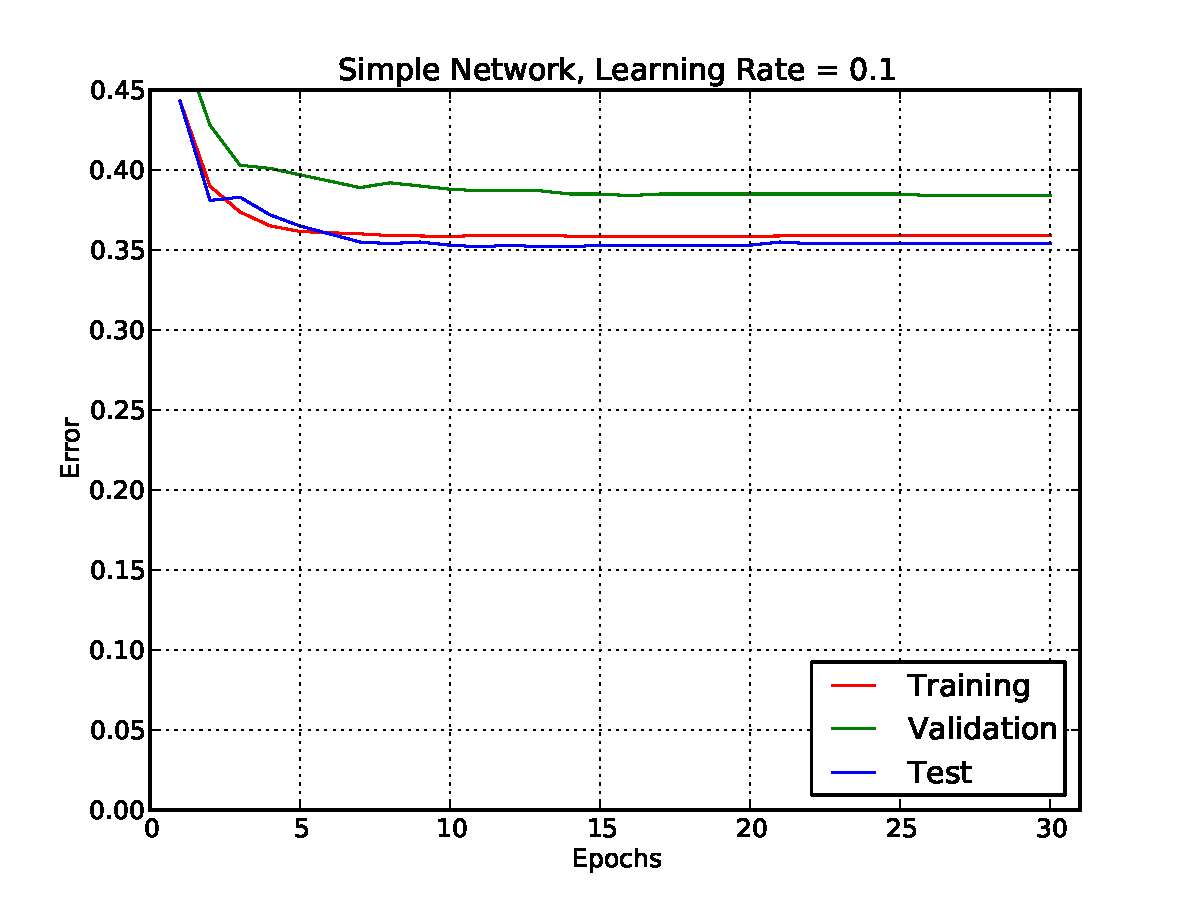
\includegraphics[scale=0.8]{source/simple-network-alpha-0_1.pdf}
\end{center}

The weights associated with this neural network were made available to our player. In order to test the performance of our player with access to this neural network, we made changes to the handout code to make it run faster and prevent the game from hanging on enter at the end of a game. These changes required removing calls to {\tt sleep} and {\tt sys.stdin.read(1)}. We then used our {\tt win\_loss\_ratio} script, called with the number of games to run as an argument (e.g., 1000). The script plays the requested number of games and records the numbers our player won, lost, and tied. This gave us a more objective measure of performance that running the game a handful of times. Using our neural network to classify images, our player improved significantly. It was able to beat the stock random player (i.e., the player using the code provided in {\tt common.py}) in 635 out of 1000 games.

\section{Finite Memory Policy}
\subsection{Motivation}
\hspace{4mm} Our neural network does not perform perfectly when classifying images. As described above, our network classifies images incorrectly with probability 0.354 (test error). The probability of the network classifying a plant incorrectly two times in a row is lower: $0.354^2 \approx 0.125$. This is where a finite memory policy becomes useful. Although it requires more than one observation of each plant encountered, a finite memory policy can help our player make the correct decision with a higher degree of confidence.

\subsection{Design}
\hspace{4mm} We chose to use a finite memory policy where $k=2$. That is, our player will only be able to remember the last 2 observations each time it selects an action. In our finite memory policy, the player continues requesting observations (i.e., classifications from the neural network) until two identical observations are made in a row. If the observations where both nutritious, then the player eats the plant. If the observations were both poisonous, the player does not eat the plant. If the observations are different, the player requests another observation.

We implemented this behavior by setting the variable {\tt nutritious\_count} to 1 if we observed a nutritious plant, and to -1 if we observed a poisonous plant. Before setting the value of this variable, we check to see if its value is already equal to the value we want to set it to. If it already equals 1, and we want to set it to 1, then the player has made two consecutive nutritious observations, and the player decides to eat the plant. If it already equals -1, and we want to set it to -1, then the player has made two consecutive poisonous observations, and the player decides to ignore the plant.

\subsection{Evaluation}
Using both the neural network and our finite memory policy, our player was able to beat the stock random player in 657 out of 1000 games. Part of this improvement certainly comes from the player making correct decisions more frequently about whether or not to eat plants. However, we believe that a large part of this improvement also comes from the reduced number of observations requested per plant. The stock random player requests 5 observations of every plant it encounters. Using the finite memory policy, our player requests an average of 2 observations. Since these observations are expensive, making fewer of them is conducive to survival.

In the same vein, note that we also implemented a finite state controller by using a counter variable. The player would decide to eat or ignore a plant once this counter crossed a certain threshold (e.g., 2). However, since reducing the number of observations made is important to survival in the game, we decided to use the finite memory policy instead. The finite memory policy requires fewer observations than the finite state controller to make a decision on a plant's type. The code for the finite state controller is commented out in {\tt player.py}.

\section{Q-Learning - DANBRO}
\subsection{Motivation}
We want to know how to make the best movement decision (i.e., action) based on our current position in the world (i.e., state).

\subsection{Design}
We defined 4 states, each depending on what happened in the last round. Our states are {\sc passed}, {\sc ate nutritious}, {\sc ate poisonous}, and {\sc seen nothing}.

We ran experiments to collect data on the distribution of plants. We did this by running 2 random, base players and recording their location every time a plant was encountered (i.e., {\tt hasPlant} was set to true). We determined the kind of plant at each location in the same way as we determined labels for the plant images, by looking at the difference in life points before and after eating the plant. For convenience, we set the plant bonus to 1, the plant penalty to 1, the starting life to 100, and the observation cost and life per turn to 0. Below are plots showing the location of nutritious plants (blue dots) and poisonous plants (red dots) in the world. The third plot shows the plot of the nutritious plants superimposed on the plot of the poisonous plants.

\begin{center}
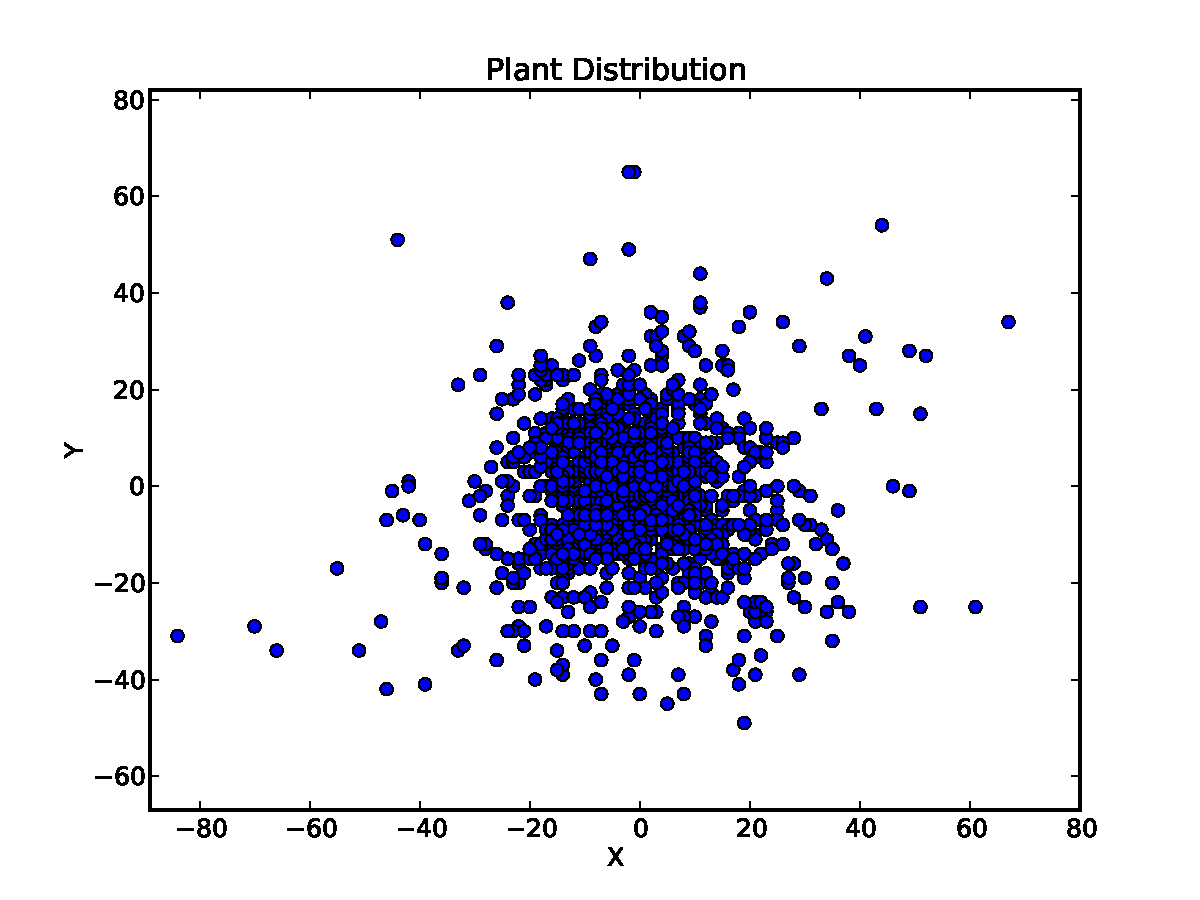
\includegraphics[scale=0.8]{source/nutritious-plant-distribution.pdf}
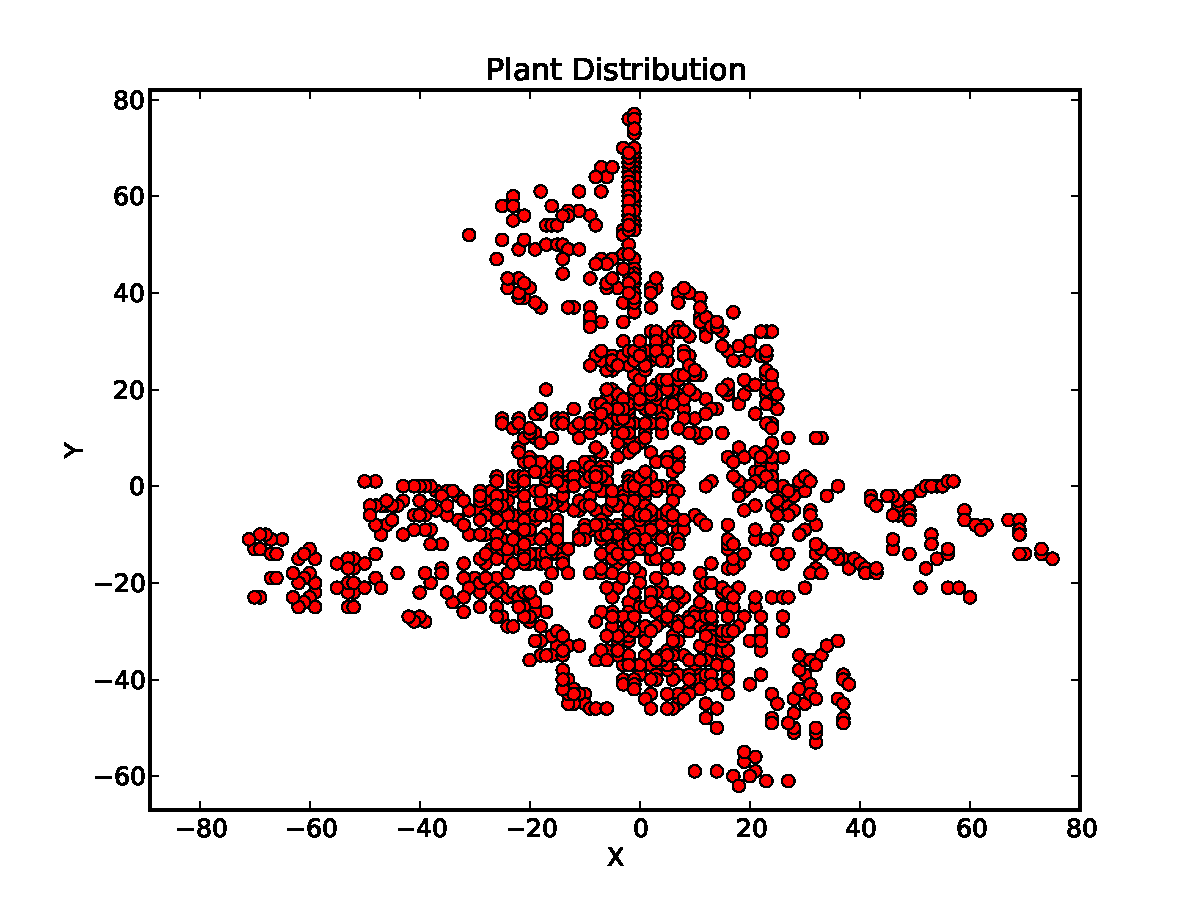
\includegraphics[scale=0.8]{source/poisonous-plant-distribution.pdf}
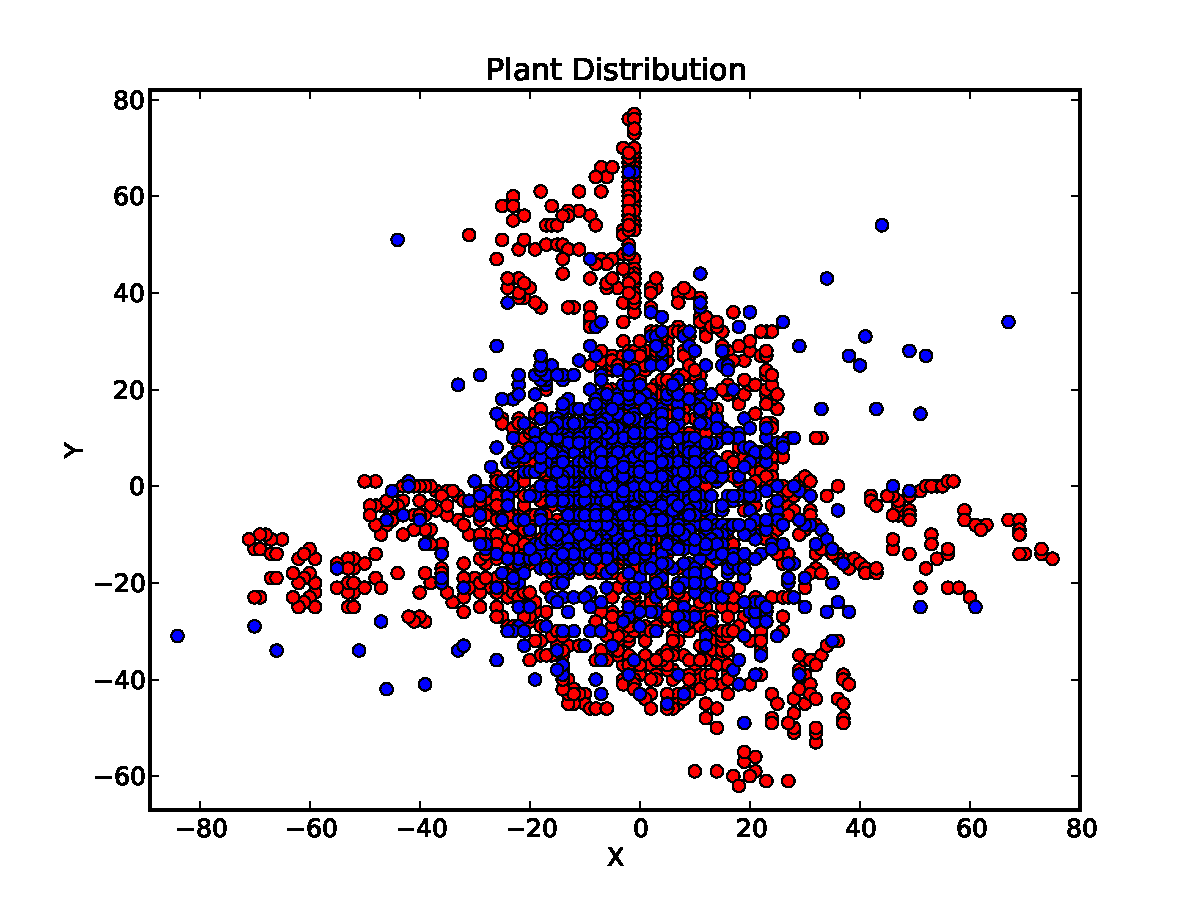
\includegraphics[scale=0.8]{source/plant-distribution.pdf}
\end{center}

The nutritious plants appear to be distributed according to a Gaussian distribution centered at the origin (mean 0) with standard deviation of approximately 20. Meanwhile, the poisonous plants appear to be distributed uniformly throughout the world. In light of this information, we designed our reward function such that moving outside of the circle centered at the origin with radius 20 is punished.

\subsubsection{Semi-Random Movement}
After making the above observations of the plant distribution, we first tried implementing a movement function which uses the {\tt GetXPos()} and {\tt GetYPos()} methods to check how far the player is from the origin. If the player is less than 20 units from the origin, the player is allowed to move randomly. Otherwise, the player is forced to take a step back towards the origin. This is done by checking if the player is more vertically or horizontally distant from the origin, and then moving the player in the appropriate direction depending on what side of the axis they are on.

\subsubsection{Q-Learned Movement}
% Remember to write about the commented out code.
\subsection{Evaluation}
Semi-random movement did not perform well. In fact, they made our player's performance worse. Using the semi-random movement technique, our player only beat the stock random player in 520 out of 1000 games.

Q-learned movement performed only slightly better. Using the Q-learned movement technique, our player beat the stock random player in 631 out of 1000 games.

After implementing our player, we discovered that the above graphs over hundreds of games actually overlap clusters of nutritious plants, making them appear normally distributed. In each game, there are actually 3-4 clusters of nutritious plants contained in the ring of radius 20 centered at the origin. As such, it would have been better if we had implemented a method like $K$-means clustering to find these clusters and move to them.



\end{document}